
\begin{minipage}[t]{\textwidth}
\Aufgabe{Ein einfaches Spiel - Aufbau des Spielfelds}

\large

Ziel in diesem Jahr wird es sein, dass alle ein eigenes Spiel programmieren. Wir beginnen nun, den Grundstein hierfür zu legen.

\vspace{0.2cm}

%%%%%%%%%%%%%%%%%%%%%%%%%%%%%%%%%%%%%%
 % FÜR NÄCHSTES MAL MODIFIZIEREN!!!
%%%%%%%%%%%%%%%%%%%%%%%%%%%%%%%%%%%%%%
 
Für unser Spiel benötigen wir 2 Klassen:
\begin{itemize}
    \item \emphColB{Spielfeld}: Enthält alle Spielfiguren und zeigt sie mit einem Bild an einer bestimmten Position an.
    \item \emphColB{Spieler}: Eine Spielfigur, die du später mit der Tastatur steuern kannst. 
\end{itemize}

\vspace{0.2cm}

Zur Bewegung des Spielers wird ein Koordinatensystem, ähnlich zu dem in Mathematik, verwendet. Es ist jedoch etwas anders. Findet folgendes (z.B. mit Google) heraus und zeichnet es unten in das Fenster mit dem Spielfeld ein:
\begin{itemize}
    \item Wie ist das Koordinatensystem ausgerichtet (insbesondere: Wo ist der Ursprung, welche x- und y-Werte haben die Ecken des Spielfelds)?
    \item Was ist eine Hitbox und wo verläuft der Rand der (angenommen rechteckigen) Hitbox des Spielers (hier als Auto im Bild)?
    \item An welchem Punkt genau sind die Koordinaten des Spielers?
\end{itemize}

\vspace{2cm}
\begin{center}
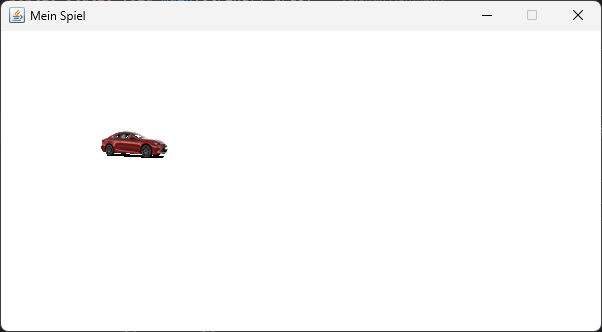
\includegraphics[width=0.9\linewidth]{_Aufgaben//BlocklyJava_Skript//img/A08_kosy.png}  
\end{center}

\vspace{2cm}

\end{minipage}

